% 2009 年湖南卷文科第 4 题：△ABC 及三边中点 D、E、F 连成的中位三角形。
% 来源 PDF：普通高考/2009/2009湖南文.pdf，SHA-256 db41a34b5d57a8db3f2ee49872e3dbc1e290c2e7390fc96cf4e084b5a679e3eb。
% 原页：第 1 页（A3 三栏）第 1 栏中部，书页码 529。
% 重绘依据：按原页相对位置重绘——A 在顶，B 在左下，C 在右下；D 在 AB 上、F 在 CA 上、
%   E 在 BC 上，三点均为中点，D-F、D-E、E-F 连成中位三角形；原页无虚实线区别。
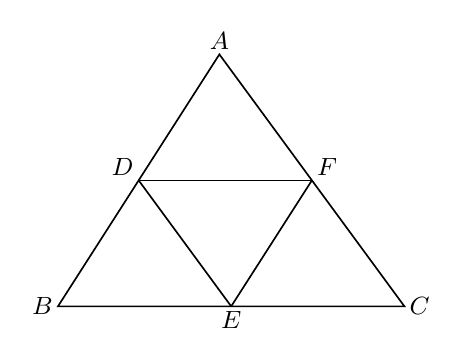
\begin{tikzpicture}[semithick, every node/.style={inner sep=1.6pt, font=\small}]
  \coordinate (A) at (2.05,3.20);
  \coordinate (B) at (0.00,0.00);
  \coordinate (C) at (4.40,0.00);
  \coordinate (D) at (1.025,1.60);
  \coordinate (F) at (3.225,1.60);
  \coordinate (E) at (2.20,0.00);

  % 三角形三边
  \draw (A) -- (B) -- (C) -- cycle;
  % 中位三角形
  \draw (D) -- (F);
  \draw (D) -- (E);
  \draw (E) -- (F);

  % 标注
  \node[above] at (A) {$A$};
  \node[left] at (B) {$B$};
  \node[right] at (C) {$C$};
  \node[above left] at (D) {$D$};
  \node[above right] at (F) {$F$};
  \node[below] at (E) {$E$};
\end{tikzpicture}
